\section{Results}
\label{sec:results}

\paragraph{Models flip at nearly twice the rate on uncertain questions (RQ1)}

\begin{table*}[t]
\centering
\caption{RQ1: Flip rates (\%) for certain ($H=0$) and uncertain ($H<0$) questions, restricted to dialogues correct at $T_0$ under the $R=3$ protocol. Pool denotes questions shared across models; $n_q^{T_0}$ counts questions with at least one correct initial response, and $n_{\text{dlg}}$ gives eligible dialogues (certain/uncertain). $\Delta$ is the flip-rate difference (uncertain $-$ certain, pp), with 95\% question-cluster bootstrap CIs (2,000 resamples). $p_{\text{Holm}}$ denotes one-sided cluster-robust logistic-test $p$-values, Holm-adjusted across 16 cells. \texttt{--} indicates missing groups or non-estimable tests due to perfect separation. $^\ddagger$ denotes a Newcombe (1998) hybrid-score CI used when identical ceiling rates yield a degenerate bootstrap CI.}
\label{tab:rq1}
\small
\begin{tabular}{llrrrrrcc}
\toprule
\textbf{Dataset} & \textbf{Model} & \textbf{Pool} & $n_q^{T_0}$ & $n_{\text{dlg}}$ (cert./unc.) & \textbf{Certain} & \textbf{Uncertain} & $\Delta$ [95\% CI] & $p_{\text{Holm}}$ \\
\midrule
MMLU-Pro & Claude Haiku & 420 & 349 & 671/277 & 89.9 & 95.3 & +5.4 [-0.2, +10.5] & 0.412 \\
MMLU-Pro & Claude Sonnet & 420 & 378 & 1014/85 & 70.8 & 83.5 & +12.7 [-1.4, +25.4] & 0.457 \\
MMLU-Pro & GPT-5.4 & 420 & 360 & 873/163 & 44.0 & 55.8 & +11.8 [-0.0, +23.3] & 0.261 \\
MMLU-Pro & GPT-5.4 Mini & 420 & 346 & 715/232 & 50.2 & 58.2 & +8.0 [-3.8, +18.7] & 0.500 \\
MMLU-Pro & GPT-5.4 Nano & 420 & 320 & 729/96 & 55.3 & 40.6 & -14.7 [-29.9, +1.3] & 1.000 \\
GPQA-Diamond & Claude Haiku & 198 & 152 & 165/208 & 98.2 & 100.0 & +1.8 [+0.0, +5.9] & -- \\
GPQA-Diamond & Claude Sonnet & 198 & 166 & 354/105 & 92.9 & 100.0 & +7.1 [+3.4, +11.0] & -- \\
GPQA-Diamond & GPT-5.4 & 198 & 171 & 366/90 & 67.5 & 68.9 & +1.4 [-14.8, +16.8] & 1.000 \\
GPQA-Diamond & GPT-5.4 Mini & 198 & 139 & 250/93 & 72.4 & 86.0 & +13.6 [-0.1, +26.2] & 0.412 \\
GPQA-Diamond & GPT-5.4 Nano & 198 & 146 & 260/65 & 59.2 & 44.6 & -14.6 [-32.8, +6.3] & 1.000 \\
HLE & Claude Haiku & 160 & 29 & 45/0 & 100.0 & -- & -- & -- \\
HLE & Claude Sonnet & 160 & 48 & 76/27 & 97.4 & 100.0 & +2.6 [+0.0, +9.4] & -- \\
HLE & GPT-5.4 & 160 & 40 & 53/25 & 88.7 & 96.0 & +7.3 [-4.8, +20.8] & 0.641 \\
HLE & GPT-5.4 Mini & 160 & 28 & 34/14 & 94.1 & 100.0 & +5.9 [+0.0, +18.2] & -- \\
HLE & GPT-5.4 Nano & 160 & 35 & 37/10 & 100.0 & 100.0 & +0.0 [-27.8, +9.4]$^\ddagger$ & -- \\
HLE & Gemini 3.5 Flash & 160 & 80 & 105/96 & 66.7 & 77.1 & +10.4 [-6.1, +27.0] & 0.556 \\
\bottomrule
\end{tabular}

\footnotesize \texttt{Reproducibility: analysis/paper\_pipeline.py}
\end{table*}

On MMLU-Pro, the uncertain group flips $46.6\%$ of the time vs.\ $23.6\%$ for the certain group when averaged across models, indicating that baseline uncertainty increases flip rate. \autoref{tab:rq1} shows this gap holds for all five included models on MMLU-Pro ($\Delta > 0$, $p < 0.001$ each). The Claude family shows the largest separation: Claude Haiku flips $28.2\%$ on uncertain questions vs.\ $0.0\%$ on certain ones, and Claude Sonnet $71.1\%$ vs.\ $10.2\%$. On GPQA-Diamond the picture compresses: Claude Haiku and GPT-5.4 have no certain group (every question elicits non-zero baseline entropy), and GPT-5.4 Mini and Nano are near ceiling on both groups ($\geq 92\%$). The certain-vs.-uncertain contrast is therefore largest on MMLU-Pro and narrows as benchmark difficulty rises; HLE, which has no certain group, is treated separately below.

\paragraph{Pressure interacts with uncertainty to predict flipping (RQ2)} \Sophia{Does it? the sign is inconsistent for Sonnet, so 25\% of the time it's different, and otherwise we don't have any evidence of interaction. I don't think we can make this claim, maybe I'm misunderstanding the figures?}
\begin{figure}[t]
\centering
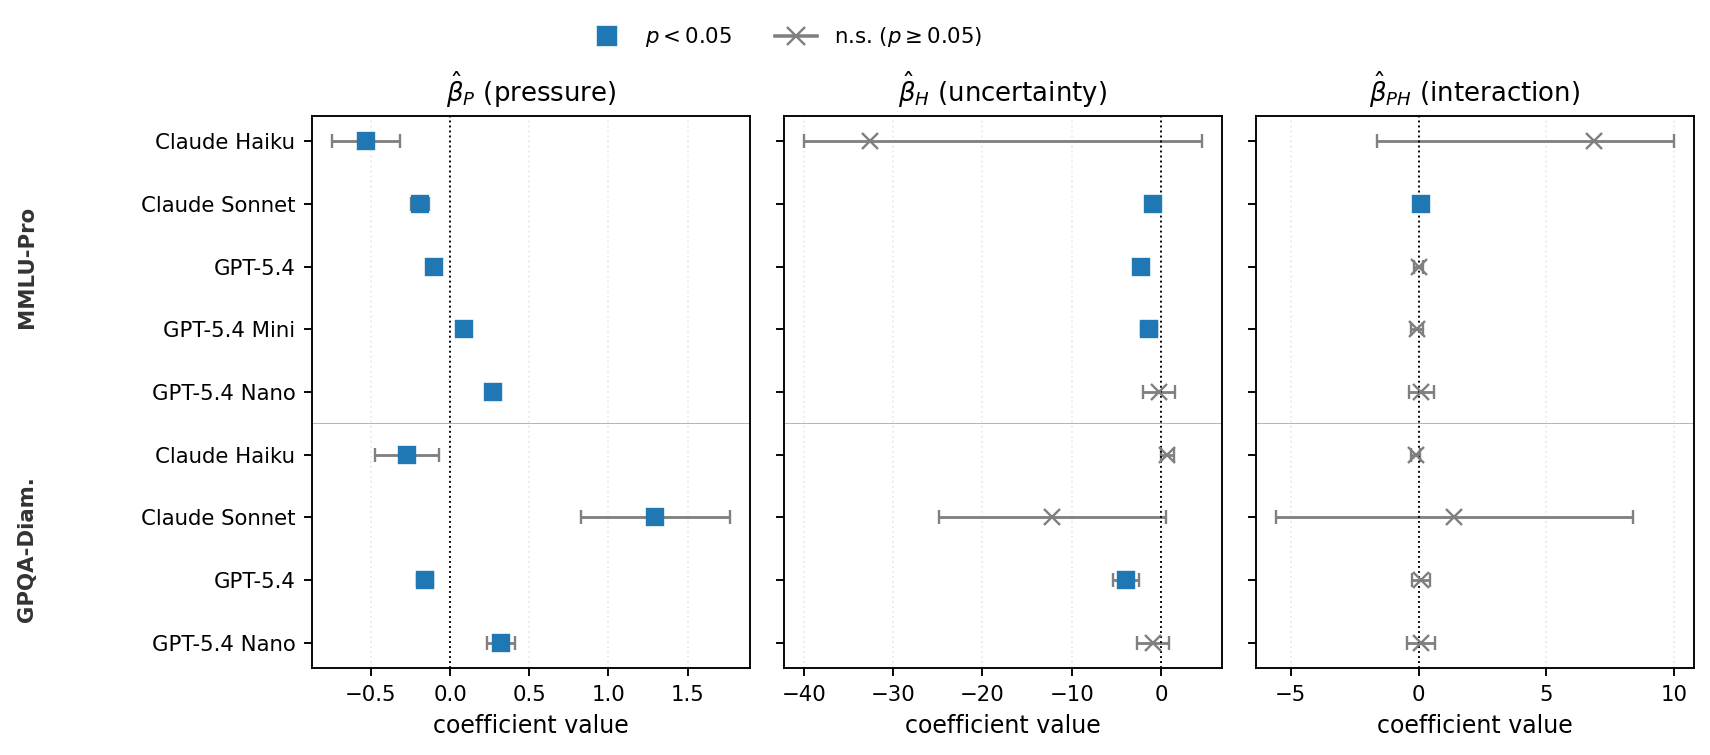
\includegraphics[width=\textwidth]{sections/fig/rq2_coefs.png}
\caption{RQ2: per-model logistic regression coefficients with 95\%  CIs. $\hat\beta_P$ (pressure main effect) sign partitions models into resisters (negative) and capitulators (positive);  $\hat\beta_H$ (uncertainty main effect) is negative in every cell where it is identifiable; $\hat\beta_{PH}$ (interaction) is significant only for Claude Sonnet on MMLU-Pro. Marker style: filled blue square = $p<0.01$, open blue square = $0.01 \leq p < 0.05$, gray cross = not significant ($p \geq 0.05$). The GPT-5.4 Mini GPQA-Diam.\ cell is omitted because of near-perfect separation; all other cells are identifiable and reported in Table~\ref{tab:rq2_combined}. Full numerical values in Appendix~\ref{app:rq2_table}.}
\label{fig:rq2_coefs}
\end{figure}

\begin{figure}[t]
\centering
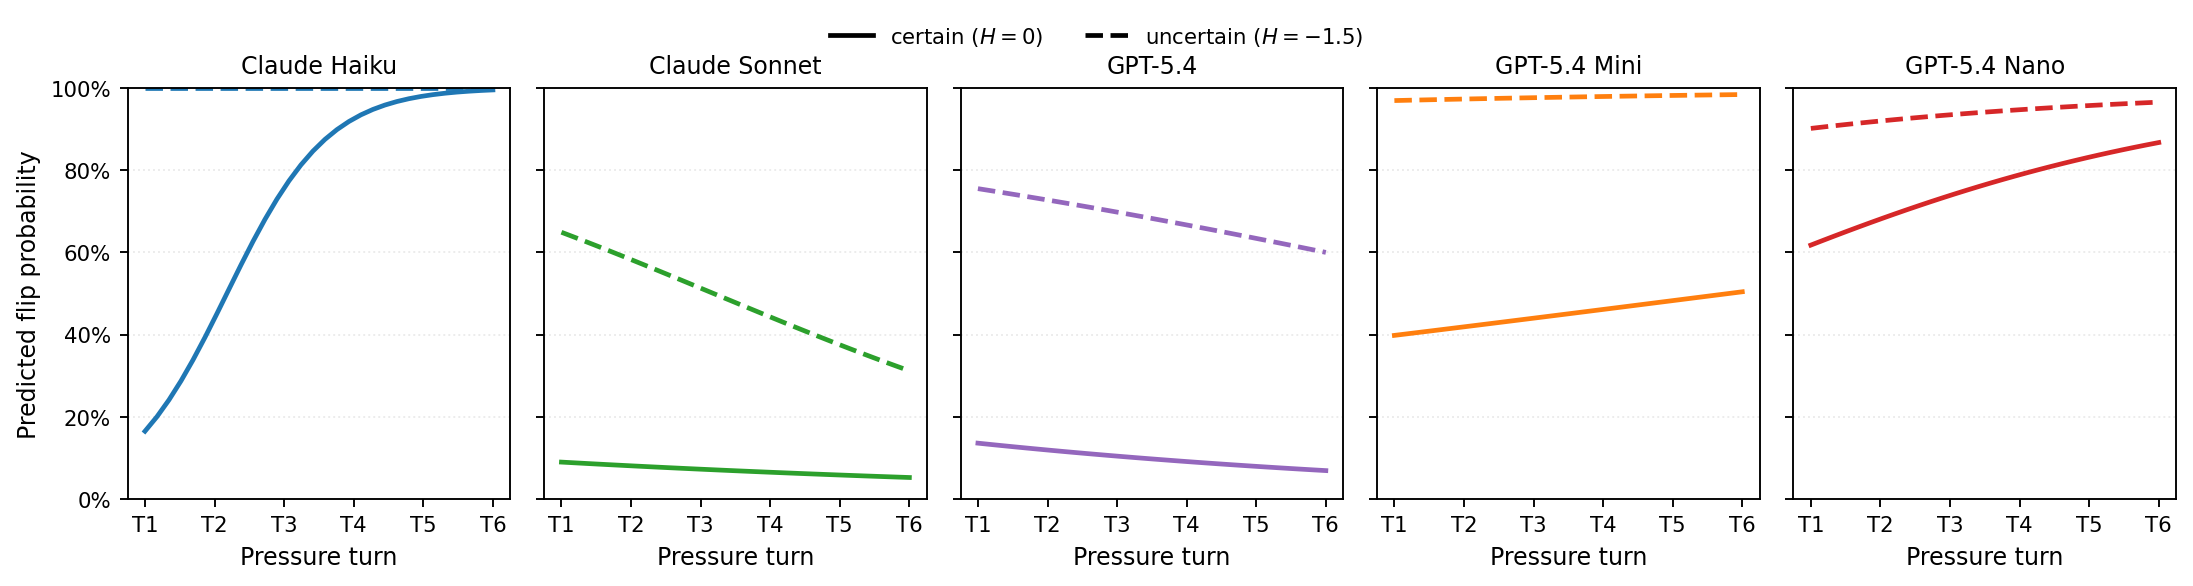
\includegraphics[width=\textwidth]{sections/fig/rq2_interaction.png}
\caption{Predicted flip probability across pressure turns
  $T_1$--$T_6$ at two uncertainty levels (solid: certain $H=0$;
  dashed: uncertain $H=-1.5$ on the raw-entropy scale) on MMLU-Pro,
  one panel per model. Curves are the fitted values from the per-model
  logistic regression of \autoref{fig:rq2_coefs}, evaluated at the
  two $H$ levels holding $P$ variable.
  The vertical gap between the two curves is the marginal effect of
  baseline uncertainty at each turn; its shape across turns
  visualizes the interaction term $\hat\beta_{PH}$. Only Claude
  Sonnet shows a clearly converging gap, matching its significant
  positive interaction coefficient.}
\label{fig:rq2_interaction}
\end{figure}


\begin{figure}
\centering
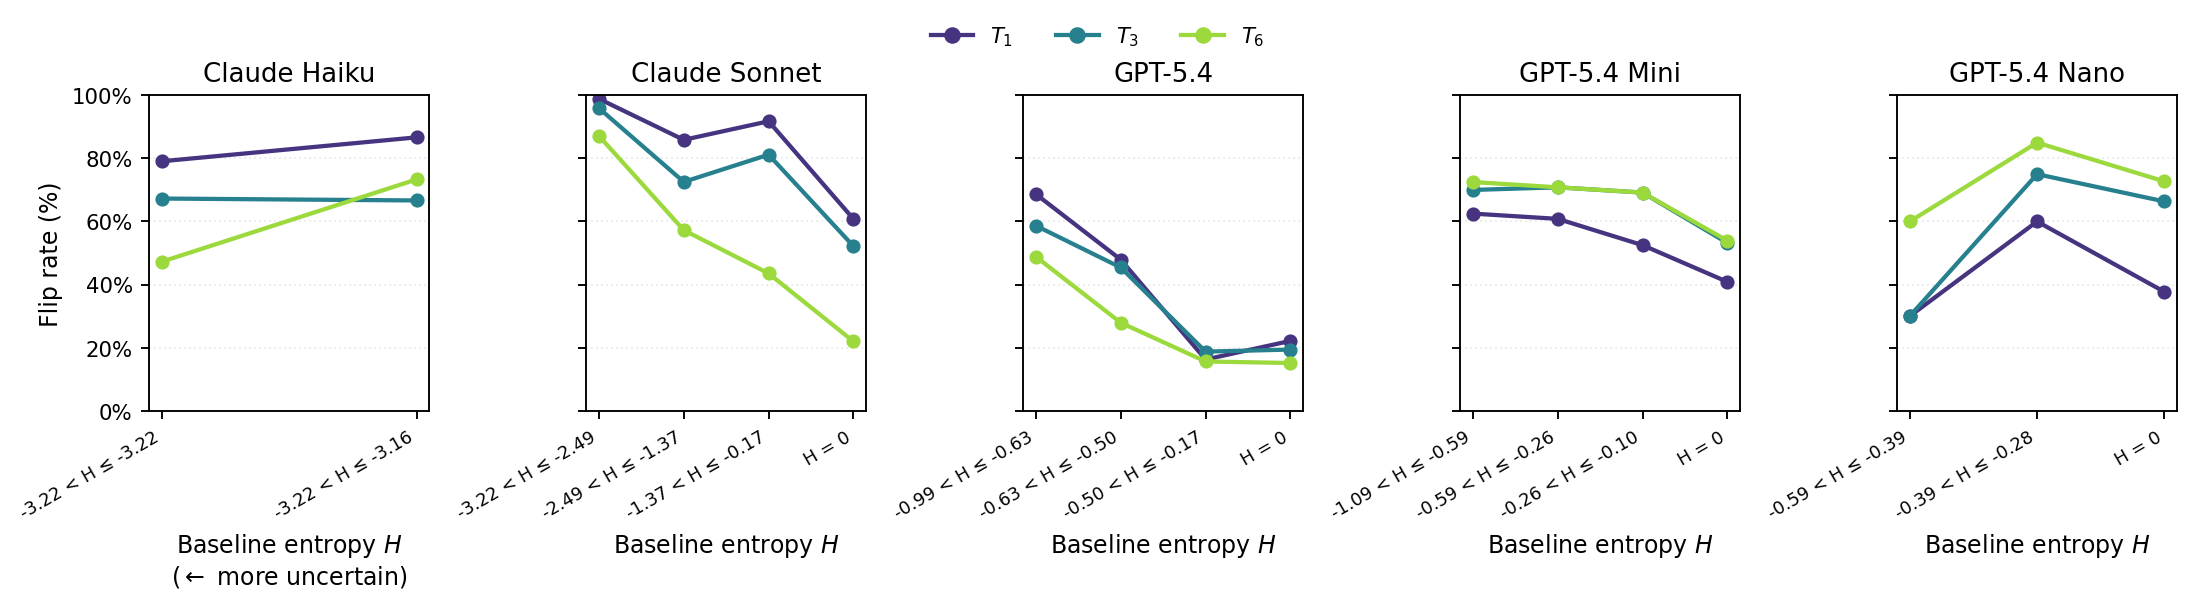
\includegraphics[width=\textwidth]{sections/fig/rq2_empirical_interaction.png}
\caption{Empirical interaction between baseline uncertainty and
  pressure turn on MMLU-Pro. Each panel: flip rate (\%) by
  per-model baseline-entropy bin, with separate lines for $T_1$,
  $T_3$, and $T_6$. Different slopes across turns indicate a
  pressure $\times$ uncertainty interaction; parallel slopes
  indicate independence. This complements the regression-based
  view in \autoref{fig:rq2_coefs} and \autoref{fig:rq2_interaction}
  by showing the raw observed pattern.}
\label{fig:rq2_empirical_interaction}
\end{figure}

\autoref{fig:rq2_coefs} shows two patterns. First, $\hat\beta_H$ is negative and significant on every MMLU-Pro cell where it is identifiable: higher baseline uncertainty raises flip probability. Second, the sign of $\hat\beta_P$ partitions models into resisters (Claude Sonnet, GPT-5.4; negative-significant) and capitulators (GPT-5.4 Mini, Nano; positive-significant). The interaction $\hat\beta_{PH}$ is significant only for Claude Sonnet on MMLU-Pro; \autoref{fig:rq2_interaction} shows this as a narrowing gap between certain and uncertain curves, and \autoref{fig:rq2_empirical_interaction} confirms the same pattern in the raw bin data. For Claude Haiku the entropy coefficient is large in magnitude but this reflects near-perfect separation on MMLU-Pro (Haiku never flips on certain questions but flips $28.2\%$ of uncertain ones), not a stronger effect: the logistic surface approaches a step function and the MLE diverges. Direction and significance are valid; magnitude is inflated.

\paragraph{Behavior under pressure varies across models (RQ3)}
\noindent
\begin{minipage}{\columnwidth}
\centering

\captionof{table}{
Per-turn flip-rate trend, cluster-robust (by question) logistic fit,
reported as the average marginal effect (AME) in pp/turn at each cell's mean
wrong rate (\autoref{sec:methods:stats}). Negative AME indicates resistance,
positive indicates capitulation; significance stars are from the underlying
cluster-robust logit slope, not the AME approximation itself.
Non-significant classifications are marked $\dagger$.
Full trajectories appear in \autoref{fig:rq3combined}.
}
\label{tab:rq3}

\small
\setlength{\tabcolsep}{3.5pt}
\renewcommand{\arraystretch}{1.04}

\begin{tabular}{@{}llcc@{}}
\toprule
\textbf{Dataset}
& \textbf{Model}
& \textbf{AME \tiny{(pp/turn)}}
& \textbf{Group} \\
\midrule

\multirow{5}{*}{MMLU-Pro}
  & Claude Haiku & $-$3.27$^{***}$ & Resister \\
  & Claude Sonnet & $-$1.32$^{***}$ & Resister \\
  & GPT-5.4 & $+$6.51$^{***}$ & Capitulator \\
  & GPT-5.4 Mini & $+$6.06$^{***}$ & Capitulator \\
  & GPT-5.4 Nano & $+$4.53$^{***}$ & Capitulator \\
\addlinespace
\midrule
\multirow{5}{*}{GPQA-Diam.}
  & Claude Haiku & $-$0.59$^{\dagger}$ & Resister$^\dagger$ \\
  & Claude Sonnet & $+$0.94$^{**}$ & Capitulator \\
  & GPT-5.4 & $+$7.85$^{***}$ & Capitulator \\
  & GPT-5.4 Mini & $+$4.21$^{***}$ & Capitulator \\
  & GPT-5.4 Nano & $+$2.53$^{***}$ & Capitulator \\
\addlinespace
\midrule
\multirow{6}{*}{HLE}
  & Claude Haiku
      & \multicolumn{2}{c}{$\varnothing$ \;\scriptsize(no reliable slope)} \\
  & Claude Sonnet & $-$0.79$^{\dagger}$ & Resister$^\dagger$ \\
  & GPT-5.4 & $+$5.30$^{**}$ & Capitulator \\
  & GPT-5.4 Mini & $+$4.85$^{**}$ & Capitulator \\
  & GPT-5.4 Nano & $+$2.47$^{***}$ & Capitulator \\
  & Gemini 3.5 Flash & $+$4.27$^{***}$ & Capitulator \\
\bottomrule
\end{tabular}

\vspace{2pt}

{\footnotesize
\emph{Significance (cluster-robust logit slope):}
$^{***}p{<}0.001$,
$^{**}p{<}0.01$,
$^{*}p{<}0.05$,
$^\dagger p{\geq}0.05$.\\
\emph{Reproducibility:}
\texttt{analysis/rq3\_rebuild.py}
}

\end{minipage}

\begin{figure}[t]
\centering
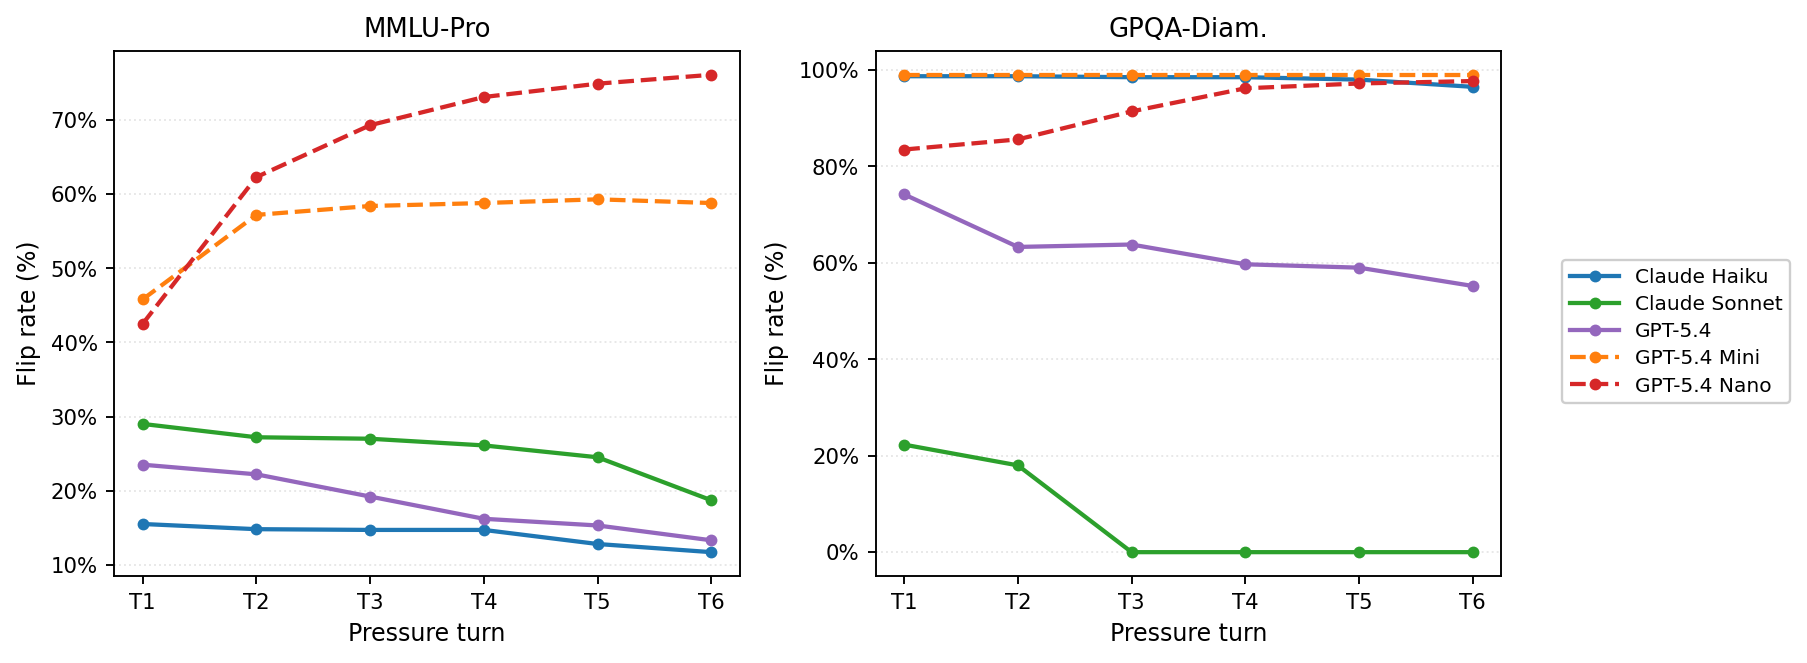
\includegraphics[width=\textwidth]{sections/fig/rq3_combined.png}
\caption{RQ3: per-turn flip-rate trajectories across $T_1$--$T_6$ for each model. Shaded bands: 95\% Wilson CIs on per-turn flip rate. The two qualitative groups are visible by slope: resisters (Claude Haiku, Claude Sonnet, GPT-5.4) decline over turns; capitulators (GPT-5.4 Mini, GPT-5.4 Nano) grow.}
\label{fig:rq3combined}
\end{figure}

Across both easier datasets, the per-model slope across $T_1$--$T_6$ partitions models into two groups. A \emph{resister} is a model whose linear flip-rate slope across the six pressure turns is significantly negative ($p < 0.05$): its susceptibility peaks at the first pressure turn and declines as pressure is sustained, consistent with early flips being partially reversed by later self-corrections. A \emph{capitulator} is a model whose slope is significantly positive: each additional pressure turn raises flip probability further, consistent with committed yielding. Claude Haiku, Claude Sonnet, and GPT-5.4 are resisters on both MMLU-Pro and GPQA-Diamond; GPT-5.4 Mini and Nano are capitulators on both.

\paragraph{Hierarchical (meta-analytic) treatment of $\hat\beta_{PH}$}
The per-model $\hat\beta_{PH}$ estimates from Table~\ref{tab:rq2_combined} show a directional split. Claude Sonnet reaches significance on MMLU-Pro ($+0.083^{**}$); the other four models are individually non-significant, with three positive point estimates (Claude Haiku $+6.885^\dagger$, GPT-5.4 $+0.002^\dagger$, GPT-5.4 Nano $+0.105^\dagger$) and one negative (GPT-5.4 Mini $-0.053^\dagger$). To assess whether the pooled interaction is robust to this heterogeneity we treat the five per-model estimates as independent effect sizes and apply standard meta-analytic tools~\citep{dersimonian1986meta}. The DerSimonian--Laird random-effects pooled estimate across all five MMLU-Pro cells is $\hat\beta_{PH} = +0.061$ ($95\%$ CI $[-0.007, +0.130]$; $p = 0.08$); excluding Claude Haiku's separation-driven estimate raises this to $+0.071$ ($p = 0.005$). The pooled interaction is therefore positive in direction but reaches conventional significance only after removing the separation-inflated Haiku cell; Figure~\ref{fig:heterogeneity} summarizes the per-model estimates and the contrast between the fixed-effect and random-effects pooled CIs. GPT-5.4 Mini's negative estimate is consistent with a ceiling effect: at baseline flip rates of $75\%$--$84\%$ these smaller models are near saturation even on certain questions, leaving little room for uncertainty to amplify susceptibility further.

\begin{figure}[t]
\centering
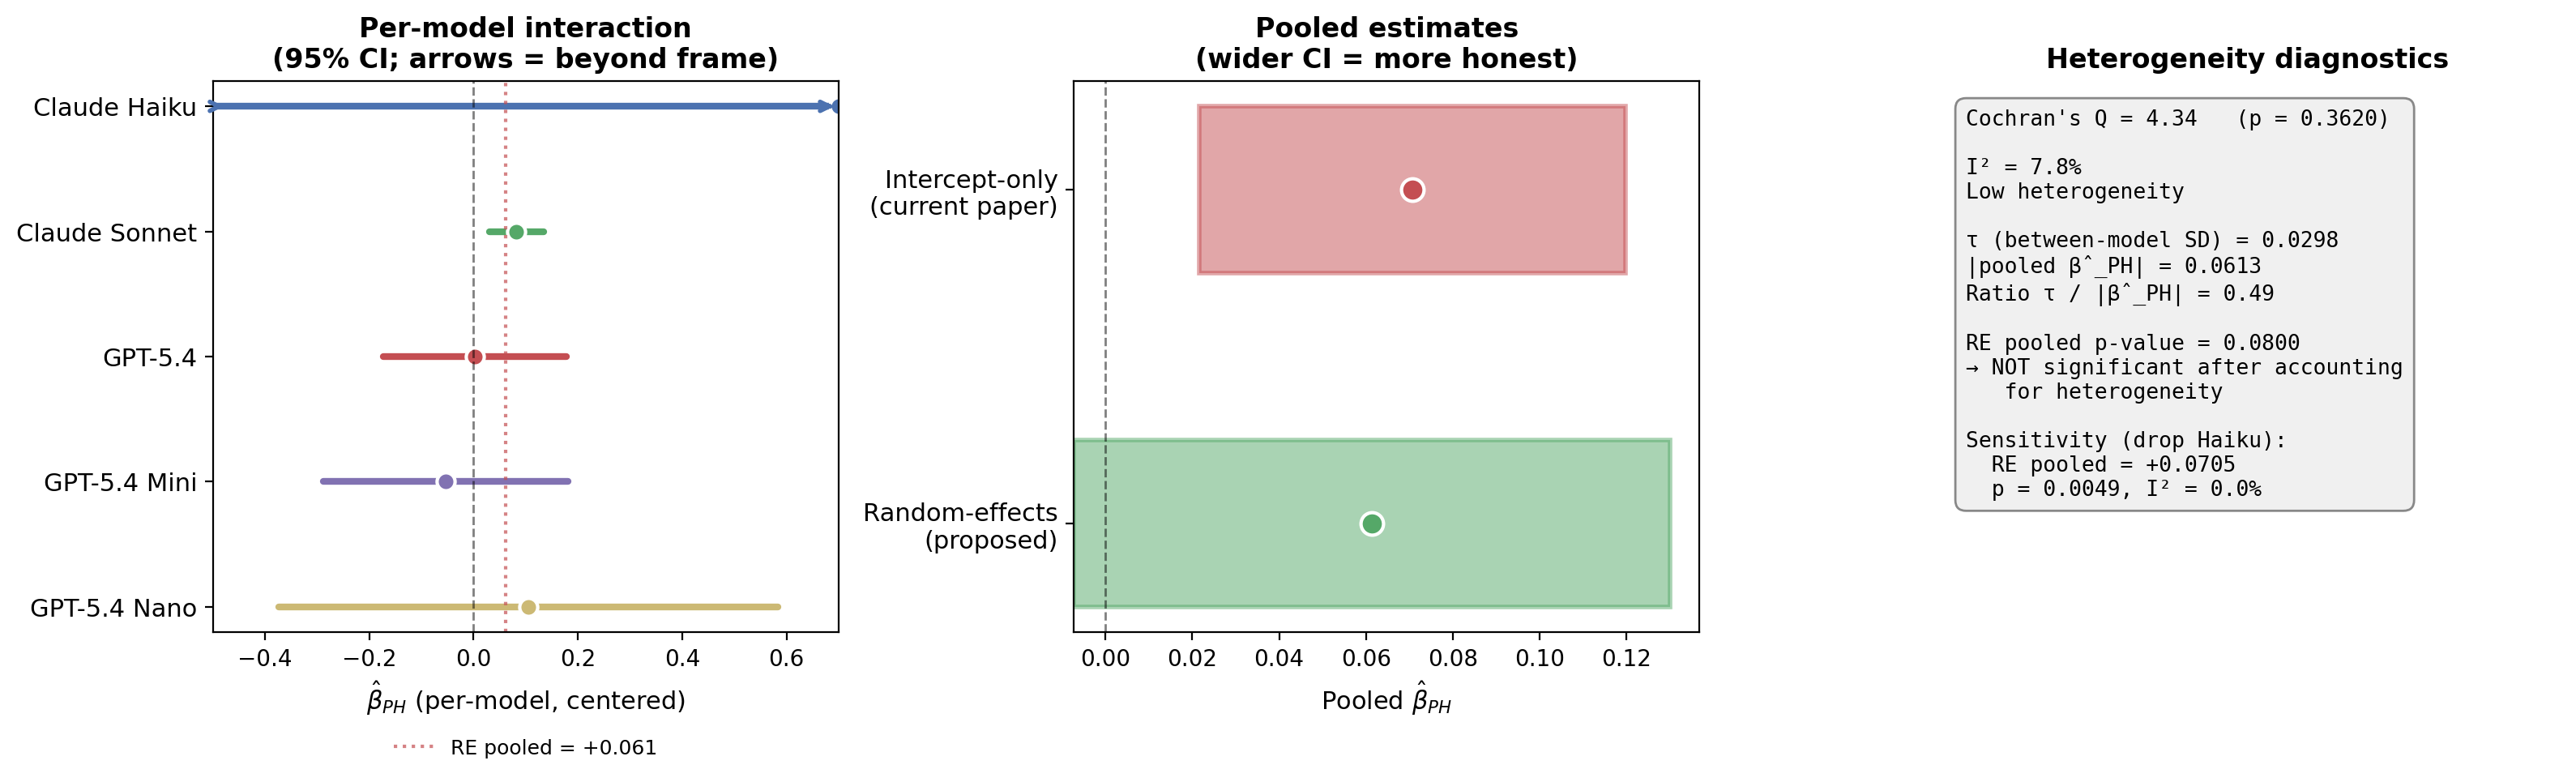
\includegraphics[width=\textwidth]{sections/fig/interaction_heterogeneity.png}
\caption{Meta-analytic heterogeneity of $\hat\beta_{PH}$ across models.
  \textbf{Left}: per-model 95\% CIs on the pressure-by-uncertainty interaction coefficient on MMLU-Pro.
  \textbf{Centre}: fixed-effect vs.\ random-effects pooled CI on all five models (RE pooled $= +0.061$, $p = 0.08$), and the same pooling excluding Claude Haiku's separation-driven estimate ($+0.071$, $p = 0.005$).
  \textbf{Right}: heterogeneity diagnostics.}
\label{fig:heterogeneity}
\end{figure}

\paragraph{HLE stress test}
We report HLE runs for all six target models. Claude Haiku has 33 $T_0$-correct queries on HLE but loses consensus on all of them by $T_2$ on average, so no per-turn flip-rate trajectory can be measured; it is excluded from the RQ3 slope analysis. The five remaining models all show \emph{positive} per-turn slopes across $T_1$--$T_6$ (Table~\ref{tab:rq3}), in the capitulator direction: GPT-5.4 Mini at $+7.59^{**}$ pp/turn, Claude Sonnet at $+6.11^\dagger$, GPT-5.4 Nano at $+2.29^\dagger$, Gemini 3.5 Flash at $+2.25^\dagger$, and GPT-5.4 at $+1.00^\dagger$. Both Claude Sonnet ($-1.73^{*}$ on MMLU-Pro, $-4.72^{*}$ on GPQA-Diamond) and GPT-5.4 ($-2.13^{***}$ on MMLU-Pro, $-3.20^{**}$ on GPQA-Diamond) are significant \emph{resisters} on the two easier benchmarks; both slopes flip sign on HLE. No HLE cell registers as a significant resister. This is consistent with the resister/capitulator classification being a joint property of (model, benchmark difficulty) rather than a fixed property of the model. Sample sizes on HLE are smaller than on the two easier benchmarks (24--72 $T_0$-correct questions per model vs.\ 400--420, driven by HLE's low baseline accuracy), so per-model point estimates carry wider uncertainty; only GPT-5.4 Mini reaches significance. Claude Sonnet's HLE trajectory is non-monotonic: flat through $T_1$--$T_3$ (flip rates $\leq 6\%$), then rising to $31\%$ at $T_4$ (expert authority) and remaining elevated through $T_6$.

\paragraph{Fragmentation is the dominant failure mode on HLE}
Consensus loss, defined in Section~\ref{sec:methods:pressure} as the turn at which no single answer wins a majority across the $R = 5$ CoT dialogues, occurs on the majority of $T_0$-correct queries for five of the six targets: Claude Haiku on $100\%$ (first loss at turn $1.91$ on average), Claude Sonnet on $98.4\%$ (turn $1.18$), Gemini 3.5 Flash on $72.2\%$ (turn $1.81$), GPT-5.4 Nano on $66.7\%$ (turn $2.56$), and GPT-5.4 Mini on $53.8\%$ (turn $2.71$). GPT-5.4 loses consensus on $21.4\%$ of $T_0$-correct queries and on average not until turn $4.33$. While on MMLU-Pro/GPQA-Diamond, fragmentation was a niche failure mode, on HLE it is the majority behavior for five of six targets. The cross-family consistency (both Claudes $\geq 98\%$; two of three GPTs above $50\%$) is consistent with a benchmark-difficulty account. The RQ4 metrics in Table~\ref{tab:rq4_hle} corroborate this: Claude Haiku's Bel.\,Ent.\ / Maj.\,Correct / Conf.\ columns are undefined from $T_2$ onward because no majority belief remains to compute them over. Discussion of practical implications for user-facing deployment is deferred to Section~\ref{sec:discussion}.

\paragraph{Belief collapses at $T_1$ while expressed confidence stays flat (RQ4)}

\begin{figure}[t]
\centering
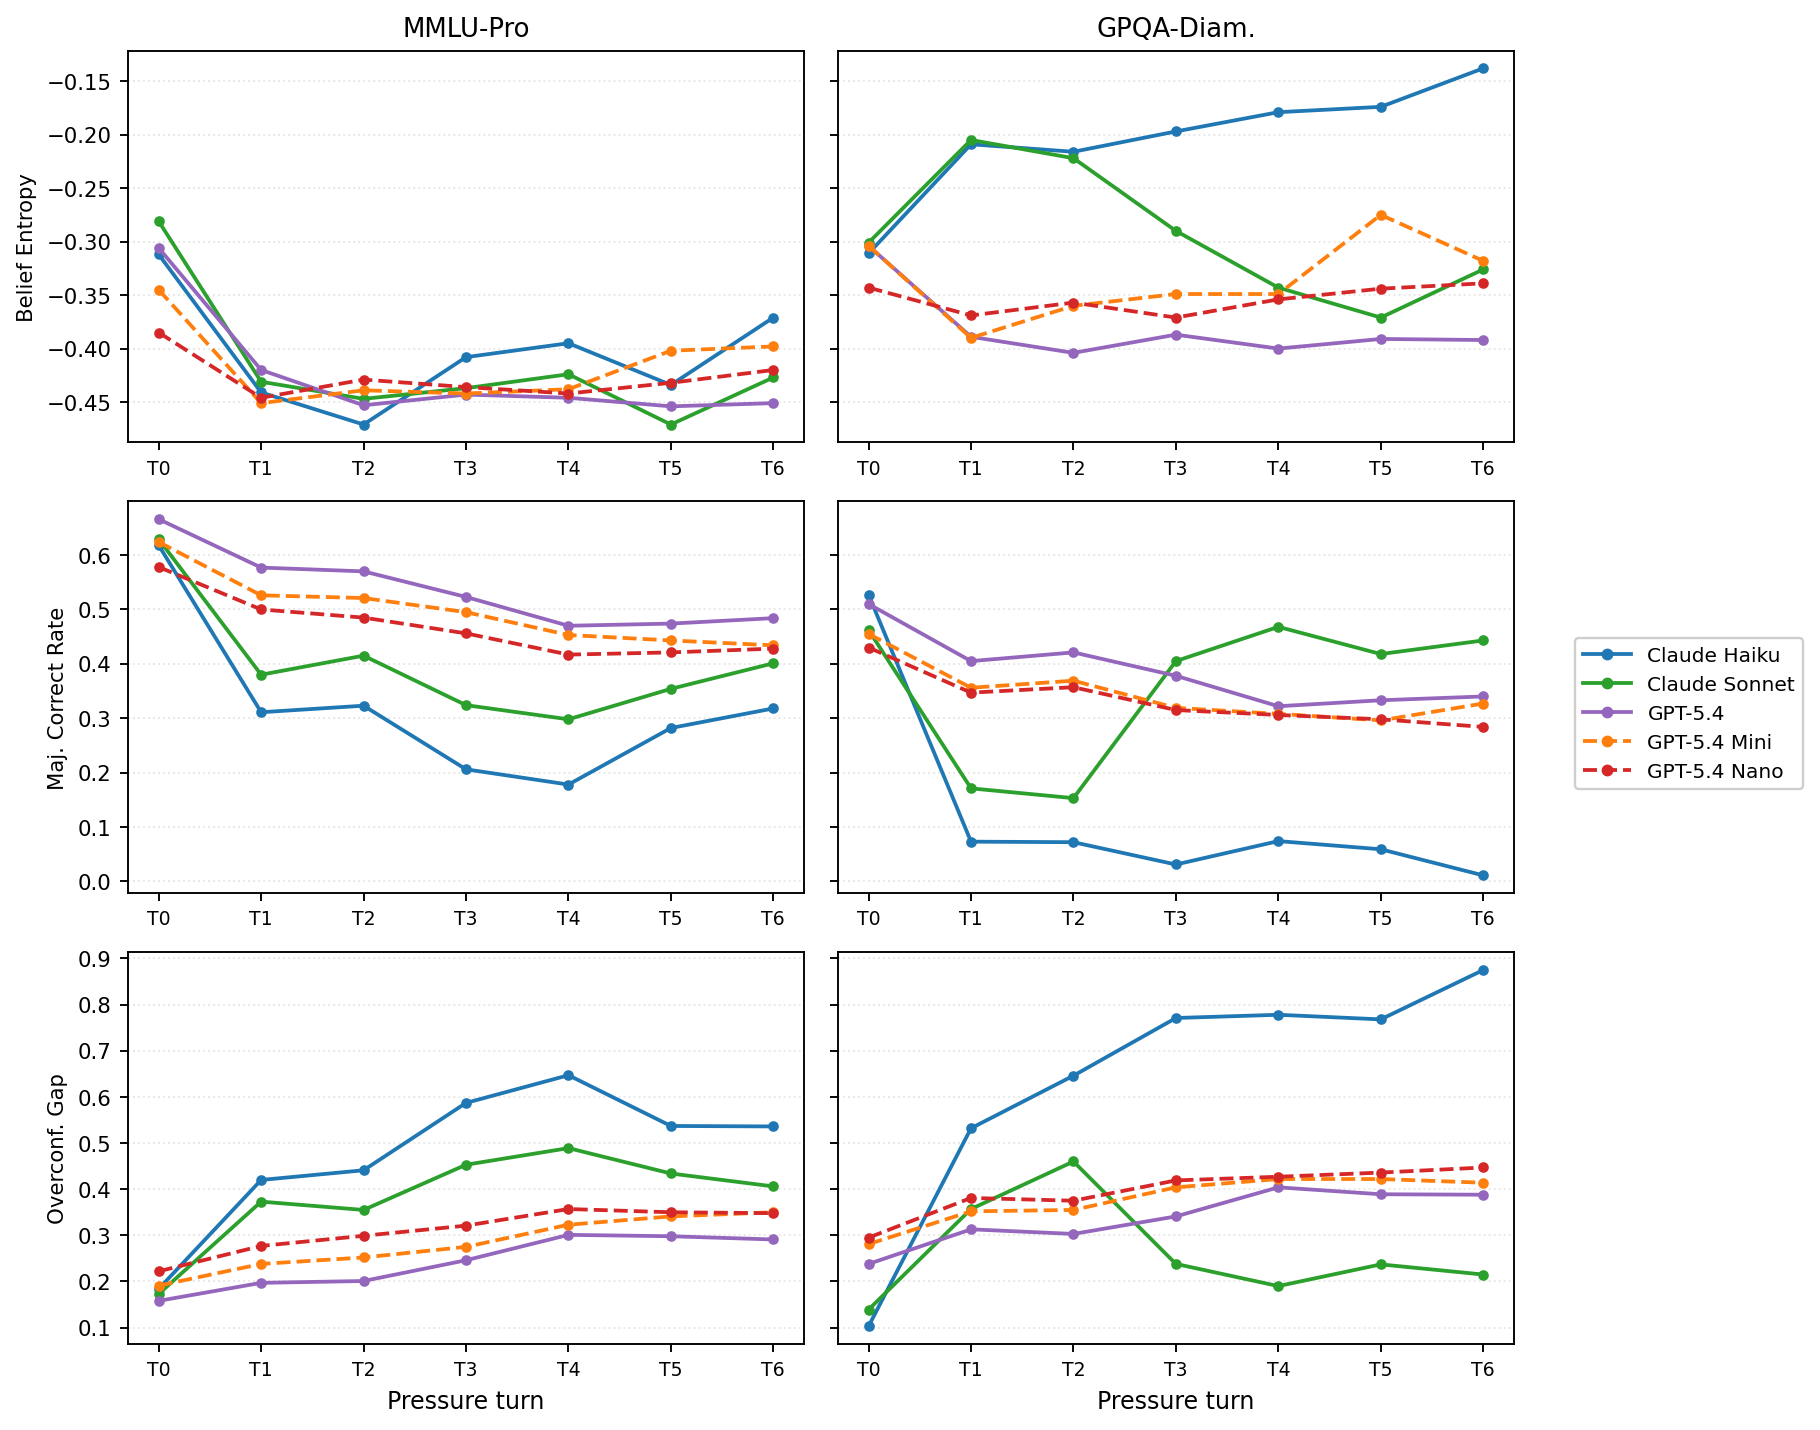
\includegraphics[width=\textwidth]{sections/fig/rq4_combined.png}
\caption{RQ4: per-turn CoT reasoning trajectories across $T_0$--$T_6$
  for each model, by dataset. Top row: majority-belief correctness (Maj.\ Correct) falls sharply at $T_1$ and stays suppressed. Bottom row: calibrated confidence (Conf.) remains nearly flat across the same turns. The dissociation between the two curves is the signature of pressure-induced miscalibration: the model's expressed confidence does not register the pressure signal even as its underlying belief collapses.}
\label{fig:rq4combined}
\end{figure}

\autoref{tab:rq4_mmlu}, \autoref{tab:rq4_gpqa} and \autoref{tab:rq4_hle} show that across all five Claude/GPT models on MMLU-Pro and GPQA-Diam., majority correctness drops $20$--$50$ pp from $T_0$ to $T_6$ while mean calibrated confidence stays nearly flat ($\pm$2--5 pp). The \emph{Gap} column (confidence minus correctness) widens correspondingly. Claude Haiku on GPQA-Diamond shows the largest gap: calibrated correctness falls from $0.527$ at $T_0$ to $0.011$ at $T_6$ while confidence rises from $0.630$ to $0.886$, a final gap of $0.875$. The intermediate turns make the trajectory visible: the gap is substantial by $T_2$ (Claude Haiku GPQA-Diamond reaches $0.646$ by $T_2$), saturates between $T_4$ and $T_5$ for most models, and stabilizes by $T_6$. The belief-entropy column shows the same trend: belief entropy becomes more negative at $T_2$--$T_6$ (more spread across the five CoT samples; recall $H \leq 0$ with $0$ = certain), so the calibrator's read of the reasoning trace becomes less stable under pressure even when the target model's expressed confidence does not.

\paragraph{Miscalibration under pressure}

\begin{figure}[t]
\centering
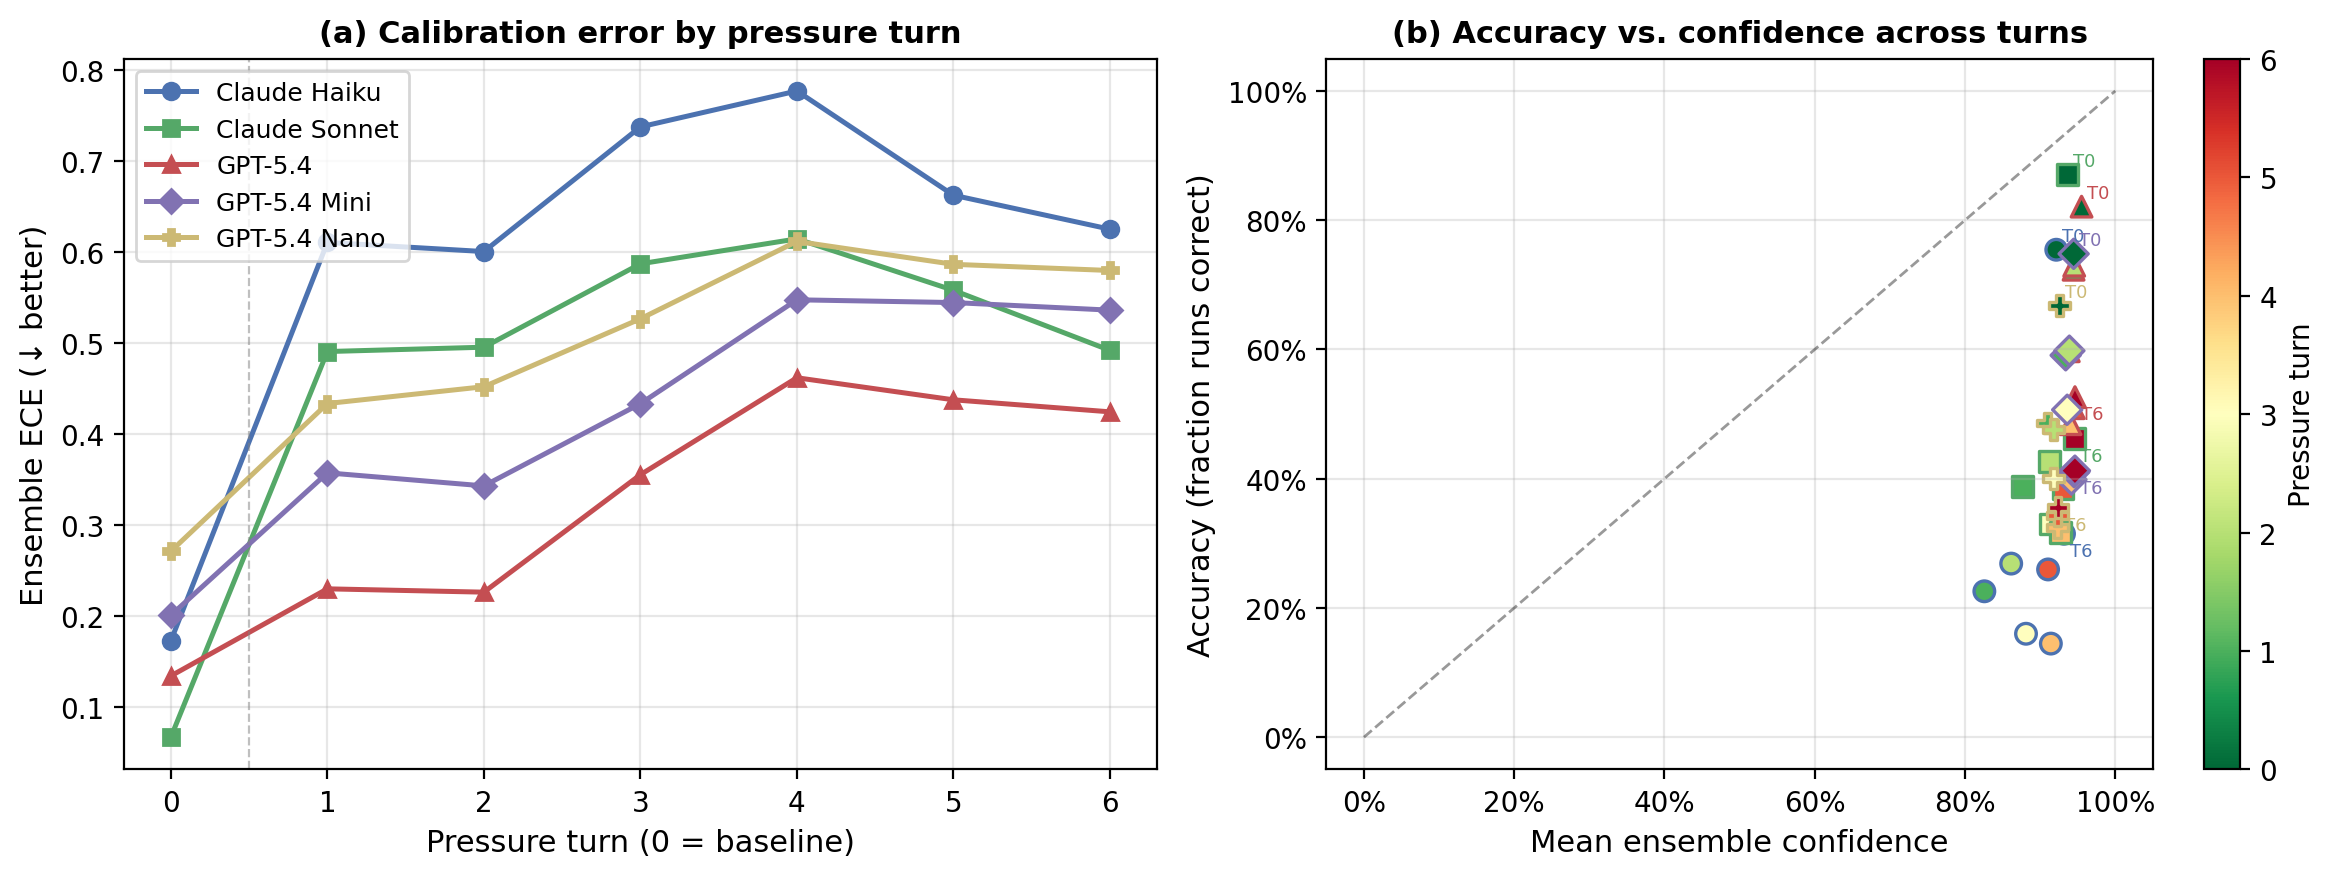
\includegraphics[width=\textwidth]{sections/fig/ensemble_calibration.png}
\caption{Ensemble calibration on MMLU-Pro.
  \textbf{(a)} Expected Calibration Error (ECE) by pressure turn for each model.
  ECE is modest at $T_0$ (0.07--0.27), then jumps at $T_1$ (0.23--0.61)
  and stays elevated through $T_6$.
  \textbf{(b)} Accuracy vs.\ mean ensemble confidence across turns $T_0$--$T_6$
  (colour encodes turn; $T_0$ = green, $T_6$ = red).
  All models lie above the diagonal at $T_0$, i.e.\ are
  overconfident even at baseline; under pressure every model
  stays at roughly the same confidence but drops in accuracy,
  widening the gap.\Sophia{This second plot is hard to read/interpret--- maybe keep just t0 and t6?}}
\label{fig:ensemble_ece}
\end{figure}

Expected Calibration Error of the ensemble confidence $\bar\gamma_{q,t}$ against per-run correctness quantifies this dissociation. At $T_0$, ECE ranges from $0.07$ (Claude Sonnet) to $0.27$ (GPT-5.4 Nano) on MMLU-Pro and from $0.11$ (Claude Sonnet, GPQA-Diamond) to $0.54$ (Gemini Flash, HLE). After the first pressure turn, ECE increases by $0.16$--$0.44$ points for every model and remains elevated through $T_6$ (\autoref{fig:ensemble_ece}a). The accuracy-vs.-confidence scatter (\autoref{fig:ensemble_ece}b) makes the mechanism explicit: mean ensemble confidence is nearly constant across $T_0$--$T_6$ (small rightward extent) while accuracy falls (large downward extent). Models do not become \emph{more} confident under pressure; they become less accurate while maintaining the same expressed confidence.

Claude Sonnet is best-calibrated overall by turn-pooled ECE (i.e., ECE computed on the full $T_0$--$T_6$ pool: $\mathrm{ECE}_{\text{pooled}}=0.47$ on MMLU-Pro, $0.24$ on GPQA-Diamond, driven by the $T_1$-onwards degradation); its ensemble confidence on GPQA-Diamond ($66.9\%$) is lower than on MMLU-Pro ($92.0\%$), consistent with greater uncertainty on harder questions. GPT-5.4 on HLE has the largest ECE ($0.85$), with an accuracy of $7.4\%$ against a mean confidence of $90.6\%$. Gemini Flash on HLE has the largest confidence--accuracy gap ($98.6\%$ confidence vs.\ $25.8\%$ accuracy, ECE $=0.73$).

\paragraph{Single-turn baseline}
To check whether the uncertainty effect of RQ1 and the pressure-category ordering of RQ3 are specific to multi-turn dynamics, we ran a single-turn pressure variant on MMLU-Pro: for each (model, question, pressure category) cell, we issue exactly one pressure prompt after the baseline answer and record whether the model flips. Two findings from the multi-turn analyses persist. First, two ordering patterns hold across all six models: expert authority is the top category, and personal certainty and crowd consensus are consistently in the bottom two. Social proof and personal disagreement occupy the middle in varying order (Appendix~\ref{app:single_turn} reports the full per-category rates). Second, the certain-vs.-uncertain gap of RQ1 persists in the single-turn regime: uncertain-baseline questions flip $30$--$80\%$ more often than certain-baseline ones, with Spearman $\rho$ between baseline entropy $H$ and single-turn flip rate in $[-0.39, -0.05]$ per model (significant at $p{<}0.05$ for Claude Haiku, GPT-5.4, and GPT-5.4 Mini). Uncertainty conditioning is therefore a property of the target model's response to social pressure generally, not an emergent effect of accumulated multi-turn dynamics.
